\documentclass[a4paper]{article}
\usepackage[utf8x]{inputenc}
\usepackage[T1,T2A]{fontenc}
\usepackage[russian]{babel}
\usepackage{hyperref}
\usepackage{indentfirst}
\usepackage{listings}
\usepackage{color}
\usepackage{here}
\usepackage{array}
\usepackage{multirow}
\usepackage{graphicx}
\usepackage{enumerate}

\usepackage{caption}
\renewcommand{\lstlistingname}{Программа} % заголовок листингов кода

\usepackage{listings}
\lstset{ %
extendedchars=\true,
keepspaces=true,
language=bash,					% choose the language of the code
basicstyle=\footnotesize,		% the size of the fonts that are used for the code
numbers=left,					% where to put the line-numbers
numberstyle=\footnotesize,		% the size of the fonts that are used for the line-numbers
stepnumber=1,					% the step between two line-numbers. If it is 1 each line will be numbered
numbersep=5pt,					% how far the line-numbers are from the code
backgroundcolor=\color{white},	% choose the background color. You must add \usepackage{color}
showspaces=false				% show spaces adding particular underscores
showstringspaces=false,			% underline spaces within strings
showtabs=false,					% show tabs within strings adding particular underscores
frame=single,           		% adds a frame around the code
tabsize=2,						% sets default tabsize to 2 spaces
captionpos=b,					% sets the caption-position to bottom
breaklines=true,				% sets automatic line breaking
breakatwhitespace=false,		% sets if automatic breaks should only happen at whitespace
escapeinside={\%*}{*)},			% if you want to add a comment within your code
postbreak=\raisebox{0ex}[0ex][0ex]{\ensuremath{\color{red}\hookrightarrow\space}}
}

\usepackage[left=2cm,right=2cm,
top=2cm,bottom=2cm,bindingoffset=0cm]{geometry}

\begin{document}	% начало документа

\begin{titlepage}	% начало титульной страницы

	\begin{center}		% выравнивание по центру

		\large Санкт-Петербургский Политехнический Университет Петра Великого\\
		\large Институт компьютерных наук и технологий \\
		\large Кафедра компьютерных систем и программных технологий\\[6cm]
		% название института, затем отступ 6см
		
		\huge Программирование\\[0.5cm] % название работы, затем отступ 0,5см
		\large Отчет по лабораторной работе\\[0.1cm]
		\large Симулятор звездной системы\\[5cm]

	\end{center}


	\begin{flushright} % выравнивание по правому краю
		\begin{minipage}{0.25\textwidth} % врезка в половину ширины текста
			\begin{flushleft} % выровнять её содержимое по левому краю

				\large\textbf{Работу выполнил:}\\
				\large Ильин А. А.\\
				\large {Группа:} 13501/4\\
				
				\large \textbf{Преподаватель:}\\
				\large Вылегжанина К.Д.

			\end{flushleft}
		\end{minipage}
	\end{flushright}
	
	\vfill % заполнить всё доступное ниже пространство

	\begin{center}
	\large Санкт-Петербург\\
	\large \the\year % вывести дату
	\end{center} % закончить выравнивание по центру

\thispagestyle{empty} % не нумеровать страницу
\end{titlepage} % конец титульной страницы

\vfill % заполнить всё доступное ниже пространство

% Содержание
\tableofcontents
\newpage

\section{Навигатор по лабиринту}
	Навигатор по лабиринту - полноценная игра, цель которой - найти выход из лабиринта. 

\subsection*{Задание}
	Необходимо написать программу, которая сможет перемещать игрока по лабиринту.
\subsection*{Концепция}
	Успешная программа будет загружать из файла лабиринт и выводить его на экран с возможностью прохождения.
	
\subsection*{Минимально работоспособный продукт (MVP)}

Консольное приложение, способное вывести на экран лабиринт, а так же перемещать игрока
\subsection*{UML-модели}
На диаграмме показано, что можно осуществить пользователю во время запуска приложения.

\begin{figure}[H]
	\begin{center}
		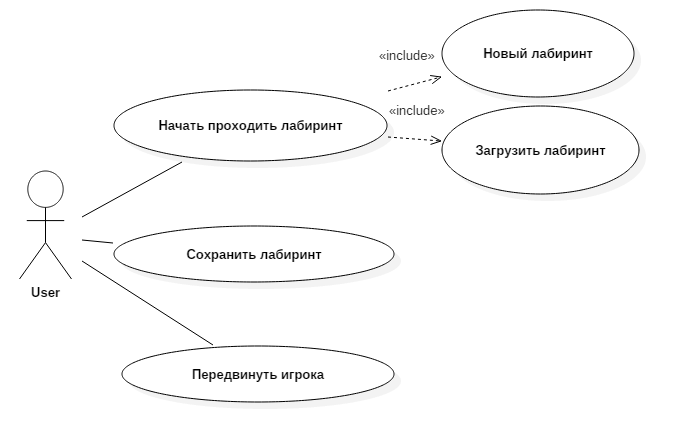
\includegraphics[scale=0.4]{UseCaseDiagram.png}
		\caption{Диаграмма прецендентов использования для интерфейса} 
		\label{pic:pic_name} % название для ссылок внутри кода
	\end{center}
\end{figure}

	
	
\section{Проектирование приложения}

Для реализации проекта использовались 2 подпроекта:

\begin{itemize}
	\item \textbf{Lib} - ядро, в котором реализованы функции, для работы с лабиринтом(является библиотекой для под проектов, отвечающих за взаимодействие с пользователем).
	\item \textbf{App} - данный подпроект был реализован с целью взаимодействия с пользователем через консоль.
\end{itemize}

\begin{figure}[H]
	\begin{center}
		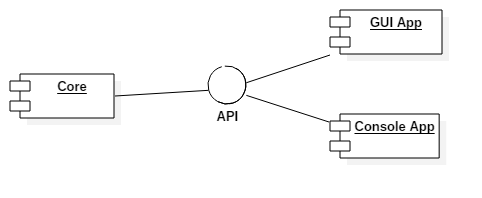
\includegraphics[scale=0.45]{Component.png}
		\caption{Диаграмма компонентов} 
		\label{pic:pic_name} % название для ссылок внутри кода
	\end{center}
\end{figure}

Библиотека предостовляет собой следующую функциональность:
\begin{itemize}

    \item\textbf{void move(std::string command)} 
    перемещение игрока по лабиринту

    \item\textbf{void fread()} 
    чтение лабиринта из файла

    \item\textbf{void findplayer()} 
    поиск игрока в лабиринте

    
\end{itemize}

	\textbf{Вывод:} Использование под проекта, как библиотеки очень полезно и удобно. 

\section{Реализация навигатора по лабиринту}
Операционная система Debian(32-bit). Для создания проекта изпользовались Qt Creator 3.5.0 (opensource) и GCC.

\subsection{Работа приложения в консоли}
	Было решено выделить один класс \textbf{App} для реализации взаимодействия с пользователем по средству консоли.
	
\section{Примеры работы придлжения}

Ниже предоставлены снимки экрана, демонстрирующие основную функциональность консольного приложения:

При открытии консольного приложения перед пользователем возникает следующее. 

\begin{figure}[H]
	\begin{center}
		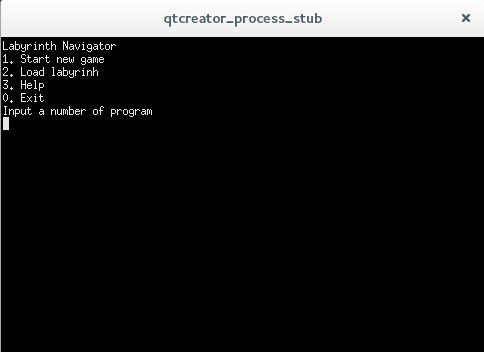
\includegraphics[scale=0.7]{Screenshot/1.jpg}
		\caption{Главное меню в консоли} 
		\label{pic:pic_name} % название для ссылок внутри кода
	\end{center}
\end{figure}

Для примера, был выбран пункт "1. Start new game". Далее пользователь может ввести команды для манипуляции над игроком

\begin{figure}[H]
	\begin{center}
		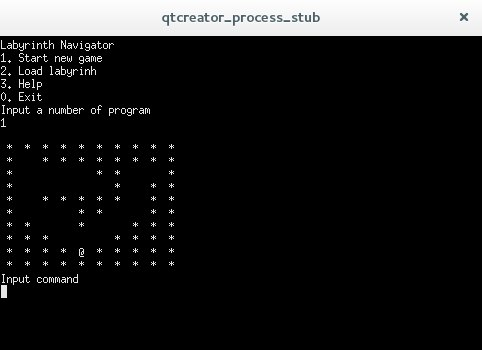
\includegraphics[scale=0.7]{Screenshot/3.jpg}
		\caption{Новая игра} 
		\label{pic:pic_name} % название для ссылок внутри кода
	\end{center}
\end{figure}

Показан пример действия комманды "up".

\begin{figure}[H]
	\begin{center}
		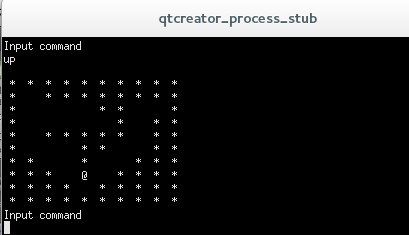
\includegraphics[scale=0.7]{Screenshot/4.jpg}
		\caption{Game command} 
		\label{pic:pic_name} % название для ссылок внутри кода
	\end{center}
\end{figure}

Показан пример действия пункта "3. Help" для предостовления помощи.

\begin{figure}[H]
	\begin{center}
		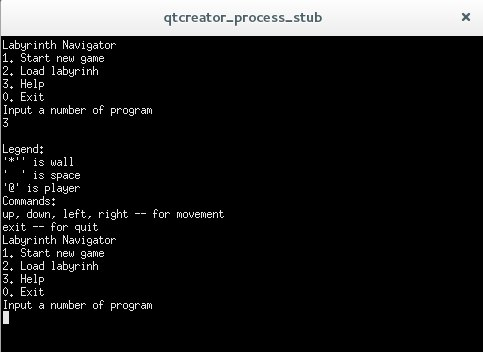
\includegraphics[scale=0.7]{Screenshot/2.jpg}
		\caption{Help Menu} 
		\label{pic:pic_name} % название для ссылок внутри кода
	\end{center}
\end{figure}


\section{Выводы}
Был написан проект "Навигатор по лабиринту", который перемещает игрока по лабиринту. Была проделана работа по созданию нескольких классов для выполнения задачи. В итоге был реализован MVP.

\section{Приложение 1}

\subsection*{Листинги}

\begin{itemize}

\item[] \verb-main.cpp-
\lstinputlisting[]
{../sources/Labyrinth_nav/app/main.cpp}
\item[] \verb-app.cpp-
\lstinputlisting[]
{../sources/Labyrinth_nav/app/app.cpp}
\item[] \verb-app.h-
\lstinputlisting[]
{../sources/Labyrinth_nav/app/app.h}

\item[] \verb-lib.h-
\lstinputlisting[]
{../sources/Labyrinth_nav/lib/lib.h}
\item[] \verb-lib.cpp-
\lstinputlisting[]
{../sources/Labyrinth_nav/lib/lib.cpp}

\end{itemize}

\end{document}